% WACV 2027 Applications Track — camera-ready.
% "Seeing but Not Speaking" (paper #949). Build: tectonic -X compile paper.tex
\documentclass[10pt,twocolumn,letterpaper]{article}

\usepackage{wacv}  % camera-ready: de-anonymised, no line numbers (WACV 2027 kit: bare \usepackage{wacv})
\usepackage{times}
\usepackage{epsfig}
\usepackage{graphicx}
\usepackage{amsmath}
\usepackage{amssymb}
\usepackage{booktabs}
\usepackage{xcolor}
\usepackage{pgfplots}
\pgfplotsset{compat=1.17}
\usetikzlibrary{calc}
\usepackage{multirow}
\usepackage{enumitem}
\usepackage[pagebackref,breaklinks,colorlinks,bookmarks=false]{hyperref}
\usepackage[capitalize]{cleveref}
\crefname{section}{Sec.}{Secs.}\Crefname{section}{Sec.}{Secs.}
\crefname{table}{Tab.}{Tabs.}\Crefname{table}{Tab.}{Tabs.}
\crefname{figure}{Fig.}{Figs.}\Crefname{figure}{Fig.}{Figs.}

% camera-ready: tighten float spacing to meet the 8-page body limit without cutting content
\setlength{\textfloatsep}{5pt plus 2pt minus 2pt}
\setlength{\floatsep}{5pt plus 2pt minus 2pt}
\setlength{\intextsep}{5pt plus 2pt minus 2pt}
\setlength{\abovecaptionskip}{4pt}
\setlength{\belowcaptionskip}{0pt}

\def\wacvPaperID{949}
\def\confName{WACV}
\def\confYear{2027}

\title{Seeing but Not Speaking: Most Token-Mass Interference in Budget-Bounded Video Question Answering Is a Decoding Artifact}

\author{Aman Verma\\
Indian Institute of Technology Bombay\\
{\tt\small 22b3929@iitb.ac.in}
\and
Anupam Rawat\\
Indian Institute of Technology Bombay\\
{\tt\small anupam.rawat@iitb.ac.in}}

\begin{document}
\maketitle

\begin{abstract}
Budget-bounded video QA methods are compared at a matched frame count, yet a choice invisible in a report of ``$K{=}16$'', the per-frame pixel budget, moves visual-token consumption by $4.2\times$ on a single answerer, and per-frame token counts at matched resolution differ by close to an order of magnitude across tokeniser families. We measure this confound and show that at a matched token budget it is the split between frame count and resolution, not the selector, that moves accuracy. Under one audited protocol (blind floors, parse health, a null beside every oracle) we map where visual-token mass helps and hurts across six Qwen checkpoints (2--8B), three further families, and seven benchmarks. A controlled decomposition appears to show that cheapening non-evidence frames is worth up to $+0.28$ accuracy while sharpening the evidence frame is worth almost nothing; this asymmetry is overwhelmingly an artifact of how the answer is read out of the model, not of visual interference. Reading the answer at the token position where the model actually emits it, rather than from free generation, removes 83\% of the effect (bootstrap 95\% CI [0.689, 1.000], $n{=}1{,}055$, 10{,}000 resamples, seed 0): on gold spans it falls from $+0.132$ ($p{=}6.2{\times}10^{-11}$) to $+0.022$ ($p{=}0.054$, paired); the residual is bounded above, not absent. The failure is expressive, not perceptual: under high token mass a susceptible checkpoint collapses to a near-constant generated answer (92\% one letter, chance accuracy) while its discriminative knowledge survives, recoverable at zero cost. A label-free diagnostic separates the susceptible checkpoint from five unaffected siblings (0.970 vs.\ 0.222--0.284; \cref{tab:collapse}); a LoRA on 0.12\% of weights also repairs it, but two thirds of that is generation, not capability. The contribution is a control and a detector, shown at one checkpoint with five siblings as negative controls. Since the generative readout is the field's default, other reported long-context visual degradations may carry the same confound; we have not tested any published result and offer this as a hypothesis the released protocol makes cheap to test.
\end{abstract}

\section{Introduction}
\label{sec:intro}

A vision--language model answering a question about video sees a handful of frames. The literature on which frames has grown quickly---keyframe scoring~\cite{tang2025aks}, tree search~\cite{wang2025videotree}, query-adaptive resolution~\cite{zhang2025qframe}, relevance--diversity retrieval~\cite{carbonell1998mmr}---and each reports gains over uniform sampling at a matched frame count $K$.

This paper argues that $K$ is the wrong unit, and, more consequentially, that the way the field reads an answer out of the model manufactures much of the effect that motivates this literature.

\noindent\textbf{The wrong unit.} Two methods reported at ``$K{=}16$'' need not consume the same visual tokens, because tokens per frame varies with resolution and with the answerer's tokeniser. We measure this spread and find it large enough that a reported win at matched $K$ is not attributable to the selection mechanism alone; we then re-measure published mechanisms on one harness and sweep the frame--resolution allocation at a matched token budget (\cref{sec:rebench}).

\noindent\textbf{The apparent harm, and what it really is.} Holding frame identity fixed and varying only fidelity, the harm axis appears to be the resolution of frames that do not contain the answer, an asymmetry worth up to $+0.28$ (\cref{sec:decomp}). We then test whether it is perceptual at all, and it is mostly not: reading the answer at the token position where the model actually emits it removes 83\% of the effect (\cref{sec:readout}). A susceptible checkpoint under high token mass stops being able to express what it knows; the knowledge is intact and recoverable at zero cost. What survives is one allocation rule: what interferes is total visual-token mass (frames $\times$ resolution), and within a fixed budget the split between more and sharper frames is set by where the evidence lives. The effect needs a native-resolution tokeniser, a susceptible checkpoint, and the generative readout, and disappears predictably when any one is removed.

\noindent\textbf{Scope.} The phenomenon is demonstrated at one checkpoint: two independent instruments (\cref{tab:ladder}, \cref{sec:decomp}) locate it there, a label-free detector separates it, and five siblings do not show it. This is a localization result with negative controls, not a law of video QA; what generalizes is the control and the detector.

\noindent\textbf{Contributions.} This is an application paper; its contributions are a mechanism, a measurement protocol, and a re-measurement of existing methods under it.
\begin{itemize}[leftmargin=*,itemsep=0pt,parsep=0pt,topsep=1pt]
\item \textbf{C1. The readout confound, and the control for it.} 83\% of the distractor-fidelity effect is an artifact of reading the answer from free generation (\cref{sec:readout}). Read at the position where the model emits the answer, the same model on the same frames gives $+0.022$ ($p{=}0.054$, $n{=}1{,}055$ paired) instead of $+0.132$ ($p{=}6.2{\times}10^{-11}$); across six readers and eighteen cells the correction zeroes the two interfering cells while reproducing 15/16 others to within $\pm0.007$. Since this readout is the field's default, other reported ``long-context'' visual degradations may carry the same confound; we supply the control and leave the test on published results to future work.
\item \textbf{C2. A failure that is expressive, not perceptual, and a gold-free detector for it.} Under high token mass a susceptible checkpoint collapses to a near-constant generated answer (92\% one letter, chance accuracy) while its discriminative knowledge survives. The collapse fraction needs no labels, separates the susceptible checkpoint from five unaffected ones (\cref{tab:collapse}), and is graded in token mass on exactly the interfering cells (\cref{sec:interference}). Detection and repair are free; a LoRA also repairs it, but two thirds of what it buys is generation.
\item \textbf{C3. Token accounting and an iso-token bake-off.} The per-frame pixel budget alone moves visual tokens by $4.2\times$ at a fixed $K$; re-measured in the correct unit, the allocation between frames and resolution dominates the choice of selector (\cref{sec:rebench}), with a decomposition isolating whose tokens matter (\cref{sec:decomp}) and a length rule confirmed out-of-sample on LongVideoBench~\cite{wu2024longvideobench}.
\item \textbf{C4. An audit protocol and its release.} Six learned lanes closed under pre-registered null-corrected gates (\cref{sec:audit}), plus blind floors, a fixed prompt layout, parse-health bounds, and the released grid, null calculators, and both readouts' per-question outputs.\footnote{Code: \url{https://github.com/NoviceCoderInfinity/seeker}.}
\end{itemize}

\section{Related Work}
\label{sec:related}

\noindent\textbf{Frame selection.} AKS~\cite{tang2025aks}, VideoTree~\cite{wang2025videotree}, Q-Frame~\cite{zhang2025qframe} and relevance--diversity retrieval~\cite{carbonell1998mmr} each score or search for frames and report gains over uniform sampling on their own stack. Because backbone, budget, resolution and prompt differ across papers, their relative merit has never been measured on common ground. We reimplement the core selection mechanism of several on one shared frame pool (\cref{sec:rebench}); these are our implementations, not the authors' systems, so we draw only relative conclusions. Q-Frame is closest to our decomposition, allocating resolution by relevance rank under a token budget, whose premise we test.

\noindent\textbf{Memory for long video.} MovieChat~\cite{song2024moviechat}, VideoAgent~\cite{wang2024videoagent} and Video-EM~\cite{wang2025videoem} vary what is stored; we vary what is spent.

\noindent\textbf{How the answer is scored.} Our central result belongs to a line of work in language modelling that the video literature has largely not absorbed. Holtzman et al.~\cite{holtzman2021surface} showed that raw-likelihood option scoring is distorted by surface form competition; Zhao et al.~\cite{zhao2021calibrate} showed that a label prior can be estimated from a content-free input and divided out, the calibration we adopt; Robinson et al.~\cite{robinson2023mcqa} showed that presenting options jointly and reading the option symbol beats cloze scoring; and Zheng et al.~\cite{zheng2024notrobust} showed that models carry a token-level prior over option identifiers strong enough to move answers under permutation.

We claim no novelty for the observation that the readout matters; our forced-choice readout is standard in that community. What we contribute is that this distortion is not a small correction in video QA but the dominant term in a published-style finding: an effect of $+0.132$ at $p{=}6.2{\times}10^{-11}$, attributed to visual interference, is 83\% readout. It escapes the usual diagnostics because the confound is induced by visual token mass, not option order or surface form: the option set is fixed and only the image budget changes, so permuting options~\cite{zheng2024notrobust} would not surface it.

\noindent\textbf{Long-context degradation.} Liu et al.~\cite{liu2024lost} showed that models use long text inputs unevenly, with the middle used least. Our positional controls (\cref{sec:interference}) test the visual analogue and find it null at $K{=}16$, pointing us away from placement toward token mass, and eventually the readout itself.

\section{Experimental Setup}
\label{sec:setup}

All arms share one SigLIP~\cite{zhai2023siglip} frame index per video (fps 0.1, duration-proportional), one answerer (Qwen2.5-VL-7B~\cite{qwen25vl}), one prompt template (answer instruction placed after the visual context; see \cref{sec:ablations}), and one pixel cap (200,704 px/frame) unless a rung sweep varies it explicitly.

\noindent\textbf{Benchmarks.} We use seven multiple-choice video QA benchmarks spanning short, localizable-evidence clips through hour-long video: NExT-QA~\cite{xiao2021nextqa}, NExT-GQA~\cite{xiao2024nextgqa} (which also supplies ground-truth evidence spans and so anchors \cref{sec:decomp}), EgoSchema~\cite{mangalam2023egoschema}, MLVU~\cite{zhou2024mlvu}, LongVideoBench~\cite{wu2024longvideobench}, the long split of Video-MME~\cite{fu2025videomme}, and LVBench~\cite{wang2025lvbench}. All are multiple choice, which is what makes the readout of \cref{sec:readout} well defined.

\begin{table}[t]
\centering
\footnotesize
\setlength{\tabcolsep}{2.5pt}
\begin{tabular}{llcc}
\toprule
family & role & \multicolumn{2}{c}{blind floor}\\
 & & NExT-GQA & EgoSchema\\
\midrule
Qwen2.5-VL-7B & primary & 0.236 & 0.232\\
InternVL3.5-8B & cross-family & 0.444 & 0.183\\
LLaVA-OneVision-7B & boundary & 0.467 & 0.138\\
\bottomrule
\end{tabular}
\caption{Zero-frame language-prior floors~\cite{li2024onevision,qwen25vl,wang2025internvl35}. Floors are not comparable across families (LLaVA-OneVision answers NExT-GQA at 0.467 with no video; Qwen2.5-VL at 0.236), so \textbf{a cross-family comparison that is not floor-corrected measures prior strength, not video understanding.} Every arm is reported against its own family's floor; the five further Qwen readers of \cref{tab:ladder} are compared only within family.}
\label{tab:floors}
\end{table}

We report accuracy with exact-binomial McNemar tests~\cite{mcnemar1947} on paired discordants and Wilson 95\% intervals~\cite{wilson1927}, at full benchmark scale. Where a quantity is a maximum over arms (an oracle, or a best-of-$N$), we never report it without its scatter null; \cref{sec:promotion} contains a case where this rule reversed a conclusion.

\noindent\textbf{Readouts.} Every table and figure states its readout: \emph{generative} (greedy generate, parse, score over parseable outputs; the field's default) or \emph{forced choice} (\cref{sec:readout}; no parse failures).

\noindent\textbf{Power and units.} An earlier round ran at $n{=}150$ ($\pm0.08$ Wilson), where headline deltas were direction-consistent but inside the interval; we re-ran every claim-carrying cell at $n{\approx}450$ ($\pm0.046$), reporting cells still inside the interval as non-significant rather than promoted. Per-frame cost is reported as visual tokens read from the processor, not pixels, since the mapping is tokeniser-specific; our ``thumb'' rung is 50,176 px and ``full'' is 200,704 px.

\noindent\textbf{Calibration.} Absolute accuracies sit below published leaderboard figures for 7B models because we study a deliberately constrained operating point (low frame rate, fixed pixel cap, no per-dataset prompt tuning). Every claim is a relative comparison between arms sharing answerer, frame set, and prompt, so a shift in operating point moves all arms together; that the operating point might itself induce collapse is why we report the boundary (\cref{sec:interference})---the same point does not collapse a stronger reader of the same family.

\section{Experiments and Results}
\label{sec:experiments}

\subsection{Token-Mass Interference}
\label{sec:interference}

Accuracy does not increase monotonically with frame budget; on short, dense clips it collapses: more frames make it worse. We establish the cause by elimination, testing each candidate at full scale.

\noindent\textbf{Not position.} If added frames displaced the evidence, accuracy would depend on where the gold frame sits. Placing a gold-span frame at controlled positions among distractors, paired within question: at $K{=}8$ the evidence is demonstrably used but every positional contrast is null; at $K{=}16$ the gold frame gives no measurable lift---drowned, not misplaced.

\begin{table}[t]
\centering
\footnotesize
\setlength{\tabcolsep}{2.4pt}
\begin{tabular}{llcccc}
\toprule
reader & dataset & cheap & costly & $\Delta$ & slope\\
\midrule
\multirow{4}{*}{Qwen2.5-VL-7B}
 & EgoSchema & 0.248 & 0.948 & $+0.700$ & $-0.290^{*}$\\
 & NExT-GQA & 0.221 & 0.418 & $+0.197$ & $-0.067^{*}$\\
 & NExT-QA & 0.220 & 0.358 & $+0.138$ & $-0.076^{*}$\\
 & MLVU & 0.388 & 0.265 & $-0.123$ & $-0.008$\\
\midrule
\multirow{2}{*}{Qwen3-VL-8B}
 & EgoSchema & 0.230 & 0.230 & $+0.000$ & $+0.064$\\
 & NExT-GQA & 0.244 & 0.228 & $-0.016$ & $+0.061$\\
\bottomrule
\end{tabular}
\caption{Collapse fraction (share of predictions on the most frequent label) at the cheapest (25,088 px) and costliest (200,704 px) rungs, $K{=}16$, generative readout, beside the resolution slope of \cref{tab:ladder}. The label-free signature rises with token mass on exactly the interfering cells and is flat or falling elsewhere: four for four within one reader, flat on the control reader. The remaining four Qwen readers of \cref{tab:ladder} are flat on EgoSchema (cheap $.236$--$.320$, costly $.226$--$.318$, $|\Delta|{\le}0.01$, slope $+.000$--$+.032$). The abstract's 0.970 vs.\ 0.222--0.284 is \textbf{not} the 0.948 cell above: it is the FF-arm collapse fraction of the four-arm decomposition on EgoSchema (\cref{sec:decomp}, retrieval proxy; $n{=}1{,}500$), Qwen2.5-VL-7B (0.970) vs.\ siblings (3B 0.245, Qwen3-VL-8B 0.222; the 2B/4B endpoints not independently reproducible from released outputs). $^{*}$ $p{<}0.05$.}
\label{tab:collapse}
\end{table}

\noindent\textbf{Not redundancy.} If near-duplicate frames drove collapse, the hardest-collapsing datasets would be the most redundant; measured directly, the prediction fails with the wrong sign (Spearman $-1.0$). Injecting redundancy at fixed token cost harms mildly, but deduplicating a collapsed context does not recover it.

\noindent\textbf{A label-free signature that tracks the harm.} The collapse fraction---the share of predictions on the single most frequent label---needs no ground truth. Swept along the rung ladder (\cref{tab:collapse}) it gives a dose--response: on the susceptible checkpoint it climbs with token mass on exactly the three datasets whose resolution slope is significantly negative and stays flat on MLVU, where that slope is null; rows one to four are the same reader, an internal control, and on the non-interfering Qwen3-VL-8B the fraction is flat everywhere. It also subsumes the length rule: on both long-video benchmarks the collapse fraction falls with added mass ($-0.261$ each), long sparse video beginning degenerate and being repaired by sharper frames. The interference and length regimes are one relation read in two directions.

\noindent\textbf{Not frame count.} Budget ladders run at low fidelity are monotone or flat: adding cheap frames does not collapse accuracy.

\noindent\textbf{It is token mass.} Holding the frame set fixed (identity verified, 80/80 exact match) and varying only the tokens each frame consumes reproduces the collapse. Across a three-rung ladder (identical 16 frames, only token mass varying) full resolution \emph{interferes} on exactly the three datasets that collapse and mildly helps on the one that does not (MLVU, $+0.044$, $p{=}0.024$); the response is not universally monotone (EgoSchema decreases, NExT-GQA and NExT-QA inverted-U, MLVU increases). Per-frame token mass has a dataset-dependent optimum, well below full resolution wherever collapse occurs; \cref{sec:frontier} resolves its location into a rule.

\begin{figure}[t]
\centering
% Bar heights from released per-question outputs: base = runs/grid_egoschema_c4_full_qwen25_7b,
% LoRA = runs/grid_egoschema_c4_full_x4control (thumb-trained, acc 0.756; matches this caption).
% See fig1_data.csv. The base-reader C bar is 458/500.
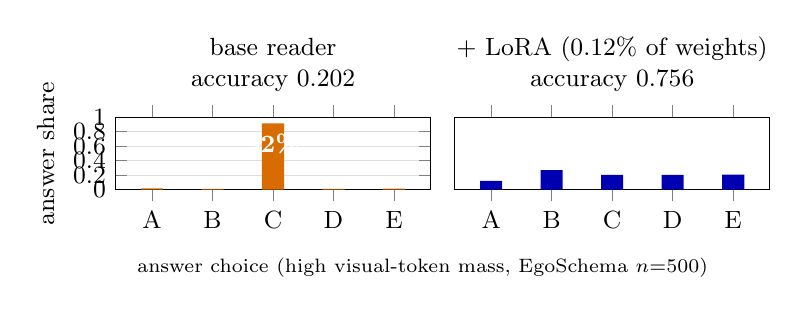
\begin{tikzpicture}
\begin{axis}[
  name=base, width=0.46\linewidth, height=2.5cm, ybar, bar width=8pt,
  ymin=0, ymax=1.0, ylabel={answer share}, ylabel style={font=\small},
  symbolic x coords={A,B,C,D,E}, xtick=data, tick label style={font=\small},
  title={\small base reader\\accuracy 0.202}, title style={align=center,font=\small},
  ymajorgrids, grid style={gray!25}, enlarge x limits=0.15]
\addplot[fill=orange!85!black, draw=none] coordinates {(A,0.018)(B,0.010)(C,0.916)(D,0.010)(E,0.014)};
\node[white, font=\small\bfseries, anchor=north] at (axis cs:C,0.90) {92\%};
\end{axis}
\begin{axis}[
  at={(base.right of south east)}, anchor=left of south west, xshift=6pt,
  width=0.46\linewidth, height=2.5cm, ybar, bar width=8pt,
  ymin=0, ymax=1.0, yticklabels={}, ytick=\empty,
  symbolic x coords={A,B,C,D,E}, xtick=data, tick label style={font=\small},
  title={\small + LoRA (0.12\% of weights)\\accuracy 0.756}, title style={align=center,font=\small},
  ymajorgrids, grid style={gray!25}, enlarge x limits=0.15]
\addplot[fill=blue!70!black, draw=none] coordinates {(A,0.120)(B,0.268)(C,0.202)(D,0.204)(E,0.206)};
\end{axis}
\node[font=\scriptsize, anchor=north] at ($(base.south)+(1.9cm,-0.75cm)$) {answer choice (high visual-token mass, EgoSchema $n{=}500$)};
\end{tikzpicture}
\caption{\textbf{The collapse is behavioural, and it is cheap to remove.} Under high visual-token mass the base reader's generated answers degenerate to a near-constant choice (92\% ``C'', accuracy 0.202 $\approx$ chance); a LoRA on 0.12\% of weights restores a healthy distribution and 0.756 accuracy \emph{regardless of the resolution it was trained on}, so we find no evidence that exposure resolution is causal.}
\label{fig:collapse}
\end{figure}

\noindent\textbf{What the collapse actually is.} A pre-registered probe on EgoSchema (which collapses hardest) settles the output-level question. At high token mass the model does not lose the ability to parse---it emits a valid choice on almost every question---but stops \emph{conditioning} that choice on the question: the answer distribution collapses onto a single label (``C'' on $458/500{=}92\%$, accuracy 0.202 $\approx$ chance), whereas at low token mass the same model answers diversely (top label 26\%, accuracy 0.488). The failure is a \textbf{discriminative mode collapse}, not a parsing artefact and not lost information.

\noindent\textbf{And it is fixable.} Is high-mass \emph{exposure} the causal variable? We apply a LoRA~\cite{hu2022lora} of 0.12\% of weights under two matched regimes, one trained on full-resolution frames, one on thumbnails only. Both restore the answer distribution and lift high-mass accuracy from 0.202 to 0.74, and the thumbnail-trained control does so as well as the full-resolution treatment (0.756 vs.\ 0.736, $\pm0.038$ Wilson at $n{=}500$). The exposure hypothesis is therefore \textbf{not supported}: what removes the collapse is task-adaptation, not exposure resolution. This rests on one training run per regime and one dataset, so we state it as first evidence, not a general fix.

\noindent\textbf{What the adapter actually buys.} \cref{sec:readout} lets us decompose that gain, revising the natural reading of \cref{fig:collapse}. Re-running both merged adapters with the forced-choice readout (EgoSchema, $n{=}150$ subset, seed 13): the base scores 0.075 generated but 0.525 forced, whereas after either adapter the two agree (0.760). So of the adapter's $+0.685$ headline, $+0.450$ ($\approx66\%$) is \textbf{repairing generation} and $+0.235$ ($\approx34\%$) is discriminative gain. Off-domain (EgoSchema$\to$NExT-QA) it is starker: the adapter drives unparseable output from 19.4\% to 0.0\% yet lands at 0.682 $\approx$ the base's forced-choice 0.677, recovering what the base could not express rather than adding knowledge. MLVU is intermediate (0.451 vs.\ base forced 0.360), so capability transfer is partial, not absent. Practitioners reporting gains from light fine-tuning on a fragile reader should separate the two.

\noindent\textbf{Cross-family boundary.} Where the signature holds is itself the finding. \textbf{Tokeniser:} only a tokeniser in which per-frame resolution moves the token count can exhibit the effect. InternVL3.5 (one 448px tile per frame) and Gemma-3 (every image forced to $896{\times}896$; verified) emit identical token counts for full and thumbnail inputs, so a ladder there is null by construction. \textbf{Capability:} within the tokeniser that \emph{can} express it, the effect is strong at Qwen2.5-VL-7B and \emph{reverses} at Qwen3-VL-8B. Budget collapse is thus a property of \emph{(native-resolution tokeniser)} $\times$ \emph{(susceptible checkpoint)} $\times$ \emph{(short, localizable evidence)}, and per \cref{sec:readout} also $\times$ \emph{(generative readout)}, rather than a law of video QA.

\noindent\textbf{Families exercised.} We exercised four families: Qwen~\cite{qwen25vl} (six checkpoints, 2--8B), InternVL3.5-8B~\cite{wang2025internvl35}, LLaVA-OneVision-7B~\cite{li2024onevision} and Gemma-3~\cite{gemma3}. On LLaVA-OneVision, whose AnyRes tiling responds differently, the contrast is flat (NExT-GQA $\Delta{+}0.006$, $p{=}0.75$; EgoSchema $\Delta{-}0.006$, $p{=}0.51$). InternVL3.5 and Gemma-3 cannot express the manipulation (tokeniser reason above); LLaVA-Video~\cite{zhang2024llavavideo} could not be served and contributes no numbers. Within Qwen the six-checkpoint sweep settles replication (\cref{tab:ladder}): under the generative readout the significant negative slope appears at exactly one checkpoint, while every Qwen3 size and the predecessor Qwen2-VL-7B is flat or positive. This is a \emph{measured contrast}, not a scaling law, and \cref{sec:readout} shows even it is mostly not about vision.

\begin{table}[t]
\centering
\footnotesize
\setlength{\tabcolsep}{1.5pt}
\begin{tabular}{lccc|ccc}
\toprule
 & \multicolumn{3}{c|}{generative (as measured)} & \multicolumn{3}{c}{forced choice}\\
reader & EgoS. & NExT-QA & MLVU & EgoS. & NExT-QA & MLVU\\
\midrule
Qwen2.5-VL-7B & $-.312^{*}$ & $-.198^{*}$ & $+.050$ & $-.004$ & $-.002$ & $-.042$\\
Qwen2.5-VL-3B & $+.000$ & $+.018$ & $+.050$ & $+.002$ & $+.025$ & $+.050$\\
Qwen3-VL-2B & $+.022$ & $-.003$ & $-.003$ & $+.018$ & $+.002$ & $-.006$\\
Qwen3-VL-4B & $+.020$ & $+.025$ & $+.064$ & $+.022$ & $+.028$ & $+.060$\\
Qwen3-VL-8B & $+.042$ & $+.032$ & $+.026$ & $+.042$ & $+.037$ & $+.028$\\
Qwen2-VL-7B & $+.032$ & $+.030$ & $+.006$ & $+.042$ & $+.023$ & $-.002$\\
\bottomrule
\end{tabular}
\caption{Accuracy change, cheapest to costliest rung (25,088$\rightarrow$200,704 px/frame, $K{=}16$), six readers, both readouts; negative = higher resolution hurts; $^{*}$ $p{<}0.05$. \textbf{Left:} under the generative readout a significant negative slope appears at exactly one of six readers, not even at Qwen2-VL-7B, the immediate predecessor of the same size, family and tokeniser. \textbf{Right:} under forced choice those two slopes go to zero, while 15/16 remaining cells reproduce to within $\pm0.007$: the correction removes the artifact and preserves what is real (\cref{sec:readout}).}
\label{tab:ladder}
\end{table}

\begin{table}[t]
\centering
\footnotesize
\setlength{\tabcolsep}{4pt}
\begin{tabular}{lcccc}
\toprule
\multicolumn{5}{l}{\emph{(a) Four arms, generative, $n{=}2{,}397$ gold-span}}\\
arm & gold & distractors & \multicolumn{2}{c}{accuracy}\\
\midrule
FF & full & full & \multicolumn{2}{c}{0.294}\\
FT & full & thumb & \multicolumn{2}{c}{0.529}\\
TF & thumb & full & \multicolumn{2}{c}{0.290}\\
TT & thumb & thumb & \multicolumn{2}{c}{0.509}\\
\midrule
\multicolumn{5}{l}{\emph{(b) FF/FT, both readouts, $n{=}1{,}055$ paired, McNemar}}\\
readout & FF & FT & FT$-$FF & $p$\\
\midrule
generative & 0.446 & 0.578 & $\mathbf{+0.132}$ & $6.2{\times}10^{-11}$\\
forced choice & 0.579 & 0.601 & $+0.022$ & $0.054$\\
\bottomrule
\end{tabular}
\caption{Resolution decomposition on NExT-GQA gold spans, Qwen2.5-VL-7B, identical frame sets across arms. \textbf{(a)} Cheapening the distractors is worth $+0.234$ (FT$-$FF, $p{=}2.9{\times}10^{-80}$) and $+0.219$ (TT$-$TF, $p{=}8{\times}10^{-75}$); sharpening the evidence is worth $+0.020$ (FT$-$TT, $p{=}0.004$) and $+0.004$ (FF$-$TF, n.s.). \textbf{(b)} 16.6\% of the effect survives forced choice (83\% removed; paired bootstrap 95\% CI [0.689, 1.000], $n{=}1{,}055$, 10{,}000 resamples, seed 0), which also \emph{raises} the harmed arm (FF 0.446$\rightarrow$0.579): the information was present all along. \textbf{Subset.} (b) is the $n{=}1{,}055$ gold-span questions scored under both readouts: the first 1,055 in canonical file order, where both arms ran to completion before the job stopped (a truncated run, not a designed split; \cref{sec:limitations}). The reported FF 0.446 conditions on the 767/1,055 parseable pairs -- the differential-dropout confound of \cref{sec:readout} -- so it exceeds the full-pool 0.294; both subsets' outputs are released.}
\label{tab:decomp}
\end{table}

\subsection{Where Resolution Belongs}
\label{sec:decomp}

If token mass is the harm, whose tokens matter: the frame containing the answer, or the frames that do not?

\noindent\textbf{Design.} On NExT-GQA~\cite{xiao2024nextgqa}, which provides gold temporal evidence spans, we construct four arms over an identical $K{=}16$ frame set per question (one gold-span frame plus fifteen out-of-span distractors), varying only the resolution of each role. Frame identity being fixed, any difference is attributable to fidelity alone, the control selection-based comparisons cannot run.

\noindent\textbf{Result.} \cref{tab:decomp}: the distractor effect is an order of magnitude larger than the evidence effect. Sharpening the frame that answers the question is worth $+0.020$, visible only once distractor interference is removed: with full-resolution distractors present it is $+0.004$, n.s.

\noindent\textbf{Reading.} Taken at face value, relevance-guided multi-resolution selection spends its budget on the wrong side of the decomposition: the gain such methods report would be attributable to demoting irrelevant frames, not promoting relevant ones. It also appears to explain the $K{=}16$ positional null of \cref{sec:interference}: the lift from gold evidence being present is $-0.004$ under full-resolution context and returns ($+0.233$) at thumb resolution. \cref{sec:readout} shows this reading---evidence out-competed for perception---is itself mostly wrong.

\noindent\textbf{Does this survive a real retriever?} The arms assign the evidence role using gold spans, which a deployed selector lacks---and that strengthens the conclusion: a selector that cannot identify the evidence frame must sharpen several candidates, paying distractor interference on the ones it got wrong, which \cref{tab:decomp} prices an order of magnitude above the benefit of getting one right. Gold-span assignment is the best case for promotion and still buys only $+0.020$.

\noindent\textbf{Does the asymmetry hold on other readers?} It does not, and the pattern is the finding. Repeating the identical four-arm decomposition on two further readers ($n{=}7{,}191$ per cell, pooling three controlled gold-frame positions): the distractor-fidelity harm is significant only at Qwen2.5-VL-7B ($+0.234$); on the weaker Qwen2.5-VL-3B all four arms sit near 0.54 and the effect vanishes ($+0.004$, n.s.; FF 0.539, no full-mass collapse to relieve); on the stronger Qwen3-VL-8B it reverses ($-0.020$, $p{=}6{\times}10^{-8}$), using full-resolution distractors productively. This is the reader boundary the ladder slope draws (\cref{tab:ladder}): two independent instruments locate the effect at the same checkpoint.

\noindent\textbf{Does it hold on other datasets?} It does. Because only NExT-GQA supplies gold spans, we extend the decomposition to two further datasets by assigning the evidence role with top-1 SigLIP retrieval (a proxy, anchored by the gold result, that also answers the retriever question above). On the primary reader the distractor-fidelity harm replicates on all three datasets: EgoSchema $+0.282$, NExT-GQA (gold) $+0.234$, Video-MME(long) $+0.100$, each $p{<}10^{-6}$, with the evidence effect $\approx0$ throughout. Its magnitude tracks how hard each dataset collapses under full mass (EgoSchema $>$ NExT-GQA $>$ Video-MME(long)): the harm is reader-specific but dataset-general. On EgoSchema the effect is explicitly a discriminative mode collapse (top label 93\% under full-resolution distractors), the failure mode of \cref{sec:interference}, so the decomposition and the probe describe one phenomenon.


\subsection{The Effect Is Mostly a Decoding Artifact}
\label{sec:readout}

Everything above measures accuracy the way the field does: let the model \emph{generate} an answer, parse it, score it. That readout is not neutral: our prompt ends by asking for \texttt{\{"answer": "<letter>"\}}, so the answer appears only if generation stays on format long enough to emit it. If high token mass degrades \emph{generation} rather than \emph{perception}, a purely expressive failure would masquerade as visual interference. We therefore re-measured with the answer read off the option-letter distribution at the position where the letter occurs (teacher-forcing the JSON prefix), holding model, frames, and prompt fixed.

\noindent\textbf{Five sixths of the effect is not visual.} \cref{tab:decomp}(b) is decisive. Under greedy generation the effect is large and overwhelmingly significant; under forced choice it is $+0.022$ at $p{=}0.054$, a surviving fraction of 16.6\% (bounded above, not absent; \cref{sec:limitations}). The repair is asymmetric in exactly the diagnostic direction: forced choice lifts the high-mass arm by $+0.133$ and the low-mass arm by only $+0.023$. The model was not failing to see; it was failing to say.

\noindent\textbf{A second, independent confound.} Greedy accuracy is computed over parseable outputs, and the arms do not drop equally: 18.7\% of FF generations are unparseable against 13.2\% for FT, differential dropout correlated with the treatment, so the greedy contrast is scored on subtly different subsets. Forced choice has none.

\noindent\textbf{It is the readout, not a readout that erases everything.} A correction that flattened all effects would be uninformative. \cref{tab:ladder} (right) rules that out across eighteen cells: forced choice leaves fifteen of sixteen non-interfering cells unchanged and collapses precisely the two that carried the interference claim.

\noindent\textbf{What we therefore claim.} The effect is \emph{real as measured} under the standard generative protocol, so the practical warning stands: at high visual-token mass a susceptible checkpoint loses most of its accuracy. But its \emph{cause} is generation fragility under long multimodal context, not competition for visual evidence. We accordingly retract the visual-interference reading of \cref{tab:decomp}; the loss is recoverable at zero cost by constrained decoding, without retraining or changing the input.

\begin{figure}[t]
\centering
% Points are the released grid values from runs/e17_curve_{nextgqa_ho,egoschema_full,nextqa_ho,mlvu_full,longvideobench_val};
% see fig2_data.csv.
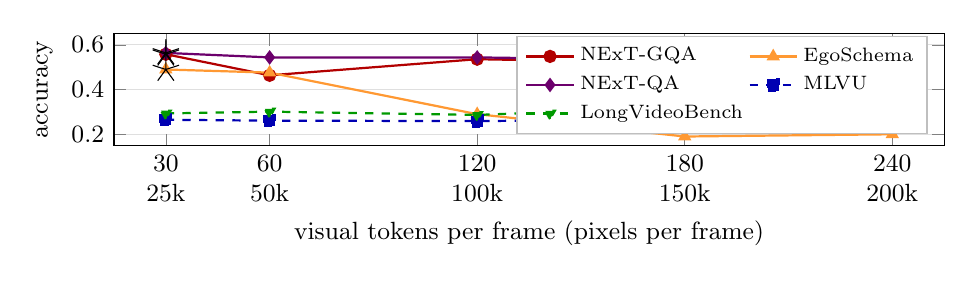
\begin{tikzpicture}
\begin{axis}[
  width=\linewidth, height=3.0cm,
  xlabel={visual tokens per frame (pixels per frame)}, ylabel={accuracy},
  label style={font=\small}, tick label style={font=\small},
  xtick={30,60,120,180,240},
  xticklabels={30\\25k,60\\50k,120\\100k,180\\150k,240\\200k},
  xticklabel style={align=center},
  ymin=0.15, ymax=0.65, xmin=15, xmax=255,
  ymajorgrids, grid style={gray!25},
  legend style={font=\scriptsize, at={(0.98,0.98)}, anchor=north east, draw=gray!50},
  legend columns=2, legend cell align=left]
\addplot[red!70!black, thick, mark=*] coordinates {(30,0.5583)(60,0.4639)(120,0.5361)(180,0.5194)(240,0.4917)};
\addlegendentry{NExT-GQA}
\addplot[orange!80, thick, mark=triangle*] coordinates {(30,0.490)(60,0.476)(120,0.290)(180,0.190)(240,0.200)};
\addlegendentry{EgoSchema}
\addplot[violet!85!black, thick, mark=diamond*] coordinates {(30,0.5642)(60,0.5441)(120,0.5441)(180,0.5315)(240,0.4887)};
\addlegendentry{NExT-QA}
\addplot[blue!70!black, thick, dashed, mark=square*] coordinates {(30,0.2649)(60,0.2610)(120,0.2590)(180,0.2669)(240,0.2689)};
\addlegendentry{MLVU}
\addplot[green!60!black, thick, dashed, mark=triangle*, mark options={rotate=180}] coordinates {(30,0.2932)(60,0.3014)(120,0.2865)(180,0.3224)(240,0.3478)};
\addlegendentry{LongVideoBench}
% optima
\addplot[only marks, mark=star, mark size=5pt, black] coordinates {(30,0.5583)(30,0.490)(30,0.5642)(240,0.2689)(240,0.3478)};
\end{axis}
\end{tikzpicture}
\caption{\textbf{The interference curve.} Accuracy against visual tokens per frame at a fixed frame count, generative readout. Solid: short, localizable-evidence datasets, which peak cheap and then fall; dashed: long, sparse video, flat or rising toward full resolution. Stars mark each dataset's measured optimum, which moves with video length and evidence density (the rule below).}
\label{fig:curve}
\end{figure}

\subsection{The Iso-Token Frontier}
\label{sec:frontier}

\cref{sec:decomp} shows fidelity has a cost. \cref{sec:interference} shows some datasets never pay it. Sweeping tokens-per-frame at a fixed frame count resolves both (\cref{fig:curve}).

Peak-low versus full is $+0.065$ ($p{=}0.029$) on NExT-GQA, $+0.292$ ($p{<}10^{-4}$) on EgoSchema and $+0.076$ ($p{<}0.05$) on NExT-QA; MLVU and LongVideoBench are flat-to-rising.

\noindent\textbf{The rule.} Short, dense clips (33--180\,s) peak at roughly 25--60 tokens per frame; long, sparse video wants full resolution. Leave-one-dataset-out, the ordinal rule recovers the measured optimum's class on 5/5 datasets; LongVideoBench is a genuine out-of-sample confirmation, not used to form the rule.

\noindent\textbf{Why we do not fit a continuous law.} A closed-form accuracy $= f(\text{tokens};\text{duration})$ is not identifiable here: the fit would have five dataset-level points, per-video duration is unavailable for three benchmarks, and where it is reliable it does not predict curation benefit (Pearson $r{=}-0.04$, $n{=}300$). Duration is an \emph{ordinal} proxy for where the optimum sits, reported as that only.

\begin{table}[t]
\centering
\footnotesize
\begin{tabular}{lccccc}
\toprule
dataset & $n$ & thumb & oracle & null & excess\\
\midrule
EgoSchema & 500 & 0.480 & 0.600 & 0.577 & $+0.023$\\
MLVU & 502 & 0.291 & 0.504 & 0.473 & $+0.031$\\
NExT-GQA & 327 & 0.502 & 0.688 & 0.670 & $+0.018$\\
\bottomrule
\end{tabular}
\caption{The ceiling of per-question fidelity allocation, generative readout. Null-corrected excess is below the pre-registered $+0.05$ bar everywhere. A small-$n$ pilot had read $+0.051$ on NExT-GQA; at full scale it is $+0.018$; the scatter null caught a false positive. Since promotion raises total token mass at $K{=}16$, this is a ceiling for policies under the generative readout, the field's operating protocol.}
\label{tab:oracle}
\end{table}

\subsection{Promotion Has No Headroom at $K{=}16$}
\label{sec:promotion}

The baseline implied by \cref{sec:decomp,sec:interference,sec:frontier} is deliberately unsophisticated: sample uniformly, render every frame cheaply, select nothing. It is training-free, sits on the iso-token frontier at fixed $K$, and the ordering holds on a second family~\cite{li2024onevision,qwen25vl}.

An obvious objection is that a smarter policy would promote a few frames to full resolution. \cref{sec:decomp} says that gain is small ($+0.020$), but not zero, so we measured the ceiling directly: for every question we enumerate all single-frame promotions (and a sample of pairs) at $K{=}16$ and take the best---an oracle no deployable policy can exceed, reported against a scatter null.

\noindent\textbf{Result.} \cref{tab:oracle}: the headroom is below bar on all three datasets before any realisation loss. Worse for the objection, a training-free policy promoting the top-1 relevance-ranked frame is significantly negative (EgoSchema $-0.050$, $p{=}0.003$; NExT-GQA $-0.058$, $p{=}0.018$), since promoting on every question pays interference on the majority where no promotion helps. The alternative's ceiling is measured, not assumed---empirical for this operating point, not a proof of unlearnability.

\noindent\textbf{Scope.} The uniform-thumbnail baseline is budget-monotone at a \emph{fixed frame count}; \cref{sec:rebench} asks how to split a \emph{fixed total budget} and finds the answer depends on where the evidence lives, so we recommend no single rendering policy. With logit access, \cref{sec:readout} makes constrained decoding the first intervention.

\subsection{Re-Measuring at Matched Token Budget}
\label{sec:rebench}

If tokens-per-frame is the controlling variable, comparisons at matched frame count are confounded. We establish that the confound is real and large, then what happens once cost is held fixed in the correct unit.

\begin{table}[t]
\centering
\footnotesize
\setlength{\tabcolsep}{4pt}
\begin{tabular}{lccc}
\toprule
configuration at $K{=}16$ & px/frame & tok/frame & total\\
\midrule
thumb rung (uniform baseline) & 50,176 & 60 & 960\\
mid rung & 100,352 & 128 & 2,048\\
full rung (default) & 200,704 & 252 & 4,032\\
\midrule
\multicolumn{3}{l}{spread from the resolution choice alone} & $4.2\times$\\
\bottomrule
\end{tabular}
\caption{Visual tokens consumed at an identical frame count, on one answerer. A choice invisible in a report of ``$K{=}16$'' moves token consumption by $4.2\times$; across tokeniser families, per-frame counts at matched resolution differ by close to an order of magnitude. Counts are read from the processor for the configurations our harness runs; we do not restate the resolutions published methods report, so the table quantifies the confound in tokens rather than auditing any single release.}
\label{tab:tokens}
\end{table}

\begin{table}[t]
\centering
\footnotesize
\setlength{\tabcolsep}{3pt}
\begin{tabular}{lccccl}
\toprule
 & \multicolumn{3}{c}{allocation (frames $\times$ tok/frame)} & &\\
dataset & $16{\times}64$ & $8{\times}128$ & $4{\times}256$ & $\Delta$ & regime\\
\midrule
\multicolumn{6}{l}{\emph{Qwen2.5-VL-7B (susceptible checkpoint)}}\\
NExT-QA & 0.539 & 0.531 & 0.642 & $+0.103^{*}$ & acuity\\
NExT-GQA & 0.478 & 0.511 & 0.625 & $+0.147^{*}$ & acuity\\
EgoSchema & 0.486 & 0.466 & 0.482 & n.s. & flat\\
MLVU & 0.277 & 0.241 & 0.253 & n.s. & flat\\
LongVideoBench & 0.299 & 0.285 & 0.274 & $-0.025^{*}$ & cover.\\
\midrule
\multicolumn{6}{l}{\emph{Qwen3-VL-8B (control checkpoint)}}\\
all five & \multicolumn{3}{c}{$|\Delta|\le0.022$} & n.s. & indiff.\\
\bottomrule
\end{tabular}
\caption{The iso-token bake-off, generative readout: one total budget (1,024 visual tokens) split three ways, paired McNemar. $\Delta = 4{\times}256$ minus $16{\times}64$; $^{*}$ $p{<}0.05$. On short, localizable-evidence datasets the susceptible checkpoint prefers acuity (four full-resolution frames beat sixteen thumbnails by $+0.10$--$0.15$); on long video coverage wins; the control reader is indifferent everywhere.}
\label{tab:bakeoff}
\end{table}

\noindent\textbf{The confound, measured.} Before comparing accuracy, we compare cost (\cref{tab:tokens}): configurations nominally at the same $K$ differ substantially in what they spend, so a win at matched $K$ is not attributable to the selection mechanism alone.

\noindent\textbf{A worked example: our own earlier result.} Before adopting this protocol we reported a selection-and-probing policy beating uniform at $K{=}8$ by $+0.064$ to $+0.130$ across three datasets, while issuing six model calls and consuming 3.96--4.00$\times$ the visual tokens. Reported as ``$K{=}8$'', that attributes to selection a gain indistinguishable from spending four times the budget.

\noindent\textbf{The bake-off.} We measure twice on the shared harness: published selection mechanisms at matched frame count, as the literature reports them, and the frame--resolution allocation at matched token budget. Pre-registered; 12/12 jobs completed.

\noindent\textbf{Frame-matched, $K{=}16$.} ``Selectors beat uniform'' is MMR-specific in our reimplementations: MMR gains $+0.050$ on MLVU and $+0.044$ on NExT-GQA, while our AKS and VideoTree are indistinguishable from uniform---a property of our reimplementations, not a failure to replicate, since we did not match the authors' full systems.

\noindent\textbf{Token-matched, and our pre-registered prediction is refuted.} At a fixed budget of 1,024 visual tokens per question, three allocations are possible by construction (px ratio 1:2:4 against frame ratio 16:8:4; \cref{tab:bakeoff}). Our prediction that many cheap frames would win is refuted on the localizable datasets, and the refutation sharpens the mechanism. On EgoSchema: sixteen full-res frames (4,096 tokens) score 0.202, chance; sixteen thumbnails (1,024 tokens) score 0.488; four full-res frames at the same budget score 0.482. \textbf{Interference is a total-visual-token-mass effect (frames $\times$ resolution), and within a fixed budget the optimal allocation is set by where the evidence lives.}

\noindent\textbf{Readout scope.} \cref{tab:bakeoff} uses the generative readout, as the literature does, which \cref{sec:readout} shows inflates contrasts at high token mass on this checkpoint; the EgoSchema 0.202 above is explicitly the collapsed arm of \cref{fig:collapse}. Every arm of \cref{tab:bakeoff}, however, sits at 1,024 total tokens, the low-mass regime where collapse is small (\cref{tab:collapse}), so we expect its acuity contrasts to be largely readout-robust; we have not verified this under forced choice (the shards record only generated answers, no logits) and read it as a statement about deployed systems under the standard readout.

\section{Ablations and Further Analyses}
\label{sec:ablations}

\noindent\textbf{Prompt layout.} Placing the answer instruction before rather than after the frames changes measured accuracy; we fix one layout (instruction last) across every arm and recommend reports state it. (No matched before/after run at fixed reader, dataset and budget is on disk, so we report this qualitatively.)

\noindent\textbf{What each benchmark actually requires.} A necessity ladder classifies every question by the cheapest resource that answers it: prior (blind correct), transcript, single frame, multi (needs the frame set, the only class a long-video claim can rest on), or unsolved. Across seven benchmarks ($n{=}86$--$1{,}337$), multi is a minority everywhere (5--26\%) and the stronger reader answers up to 56\% of a ``video'' benchmark from the language prior alone, so these benchmarks mostly do not measure video understanding. The fragile fraction falls 2--6$\times$ from the weak to the strong reader (51\%$\rightarrow$8\% on EgoSchema), recovering the boundary of \cref{sec:interference} with an independent instrument.

\section{Audit and Reproducibility}
\label{sec:audit}

\noindent\textbf{Six closed lanes.} The strongest evidence that the uniform-thumbnail baseline is right at $K{=}16$ is that we repeatedly tried to beat it with a learned policy, under gates fixed in advance, and could not. Every ceiling is quoted against its null. Selection (beat uniform at matched tokens): $-0.016$, closed. Writing (best-of-6~\cite{chen2021codex} $-$ greedy $\ge +.05$): $-0.029/+0.036$ null-corrected, closed. Routing (pooled LODO AUROC $\ge 0.75$): AUROC 0.942, yet accuracy never exceeds the best fixed policy; SPLIT. Voting (self-consistency~\cite{wang2023selfconsistency}, $+0.03$ on $\ge2$ datasets): $+0.005$ to $-0.037$, closed. Allocation and promotion (null-corrected $\ge +0.05$): $+0.018$ to $+0.039$, closed.

The writing lane is where the discipline earned its keep: a raw best-of-6 headroom of $+0.209$ would have licensed a training run, but against a chance null of $+0.239$ the excess is $-0.029$. What a policy would need is either already exploited by uniform coverage or absent from the signals, which is why the intervention that works (\cref{sec:readout}) acts on the readout, not context construction.

\noindent\textbf{Compute.} The grid (six readers $\times$ seven benchmarks $\times$ five rungs $\times$ two readouts, plus decomposition and bake-off arms) ran on single-GPU SLURM jobs (NVIDIA A40 for the harness grid, NVIDIA A100-SXM4-80GB for LoRA training), bf16, at least $\approx$124 GPU-h (a lower bound: summed wall-clock from the 395/770 \texttt{slurm-*.out} logs with a parseable timestamp pair, one GPU per job); each LoRA: rank $r{=}16$, $\alpha{=}32$, targets \{q,k,v,o\}\_proj, lr $10^{-4}$, 379 steps, effective batch 8, $\approx$2.1 GPU-h for the two full training runs (single A100).

\noindent\textbf{Controls and release.} Blind floors are at or below chance on the sets carrying our claims (\cref{tab:floors}); parse health is reported beside every many-image arm; no oracle is quoted without its null (five times; once it reversed a conclusion, \cref{sec:promotion}). We release the iso-token grid, firewall splits, null calculators, modality labels, and both readouts' per-question outputs as \textsc{TokenBudgetBench}.

\section{Limitations}
\label{sec:limitations}

\noindent\textbf{The mechanism is expressive.} We locate the failure at the output distribution, not inside the model: the probe in \cref{sec:interference} shows mode collapse rather than parsing failure or lost information, and \cref{sec:readout} recovers 83\% of the loss from the identical forward pass. That largely excludes the attention-dilution account we previously favoured: were the evidence out-competed for attention, no readout change could recover it. Why this checkpoint and not its five siblings we cannot say; a direct attention intervention is the natural next experiment. A residual $+0.022$ ($p{=}0.054$) survives correct decoding and may be a small genuine interference term: underpowered rather than shown absent.

\noindent\textbf{An alternative reading.} A narrower explanation fits the same evidence: the checkpoint loses structured-output format-following under high token mass, not generation-conditioning in general, and our JSON prompt does not separate the two. But most collapsed outputs are well-formed and merely constant (92\% one letter), a conditioning failure, not a formatting one. A bare-letter prompt ablation is the direct test; we did not run it.

\noindent\textbf{Other limitations.} The collapse regime is confirmed on one family, at one checkpoint; the five siblings are negative controls, not evidence of generality. The gold-span decomposition is single-dataset; the two-dataset extension uses a retrieval proxy. Hour-long video remains hard (on LVBench every arm sits near the blind floor). Forced choice needs logits, so it is unavailable through a text-only API, where practitioners should report parse rates per arm.

\section{Conclusion}
\label{sec:conclusion}

Budget-bounded video QA has been measured in the wrong unit and read out so as to manufacture much of what it measures. Counting cost in tokens exposes a $4.2\times$ spread inside one ``$K$''; reading the answer where the model emits it removes 83\% of the interference on the susceptible checkpoint---which does not stop seeing, it stops speaking.

{\small
\bibliographystyle{ieeenat_fullname}
\bibliography{refs}
}

\end{document}
